\section{Limitations of Existing Stream Management Techniques}
\subsection{No Automatic Stream Management for General I/O Workloads}
\begin{table}[h]
	\caption{Limitations of existing schemes}
	\label{tab:limitation}
	\begin{center}
		\begin {tabular}{cccc}
		\hline
                   		& automatic & adaptable & general workload \\
		\hline \hline
		Manual Stream   &    x      &    x      &    o    \\
		\hline
		vStream         &    x      &    o      &    o    \\
		\hline
		AutoStream      &    o      &    o      &    x    \\
		\hline
	\end{tabular}
\end{center}
\end{table}

Table~\ref{tab:limitation} summarizes the limitations of existing techniques. 
In manual techniques, developers can allocate proper streams while the stream 
allocation should be modified whenever the application or the device changes.
On the other hands, automatic technique is flexible
but it does not work well under the workload where the data lifetime is 
difficult to predict.
The detailed limitations will be explained in the following subsections.
%Our goal in this paper 
%#is to develop a fully automatic technique for general workload
%so that all the requirements are met.


\subsubsection{Manual stream management techniques}

The original design of a multi-streamed SSD can have more
than one open stream maintained inside the device, while the
application layer manages the stream open/close and maps data to an appropriate stream
~\cite{MultiStream, Level, vStream}.
Application developers assign stream ID based on their knowledge of
data temperature through a system call and the operating
system passes a stream ID down to the device. However,
this approach assumes the application developer is aware of the data
temperature and the stream related device information. 
Although \textsf{\small FStream}~\cite{FStream} does not require application modification,
they separate only file system metadata and can not separate application data without 
knowledge for data temperature such as log files of Cassandra are short-lived.
Furthermore, these manual techniques except \textsf{\small vStream}~\cite{vStream} assume 
that the number of streams in an SSD is not changing, 
thus requiring manual modifications whenever the number of streams in the SSD changes.
In order to handle the limitations of manual techniques, an automatic stream management
technqiue which can avoid the application modification and adapt the number of stream change
is highly required.
Recenlty, AutoStream~\cite{AutoStream} is proposed to automatically manage streams 
based on the data lifetime prediction with the access frequency of LBAs.

\subsubsection{LBA-based automatic technique's problems}
Many existing data separation techniques such as~\cite{HotCold, AutoStream} 
estimate the data lifetime based on the access frequency of LBAs.  
For example, \textsf{\small AutoStream}~\cite{AutoStream} assumes that, if
some LBAs are frequently accessed by applications, those LBAs hold hot data.
This LBA-based lifetime prediction 
approach, however, does not work well with recent data-intensive 
applications where a majority of
new data are written in an append-only manner.  

In order to illustrate a mismatch between an LBA-based predictor and 
append-only workloads, we analyzed the write pattern of 
RocksDB~\cite{RocksDB}, which is a
popular key-value store based on the LSM-tree algorithm~\cite{LSM}.
Fig.~\ref{fig:lba_lifetime}(a) shows how LBAs may be related 
to data lifetimes in RocksDB~\cite{RocksDB}.  
The lifetime of data in this paper is defined 
by the logical time which is the number of writes to the device 
between when the data is first written 
and when the data is invalidated by an overwrite or a TRIM command.
As shown in Fig.~\ref{fig:lba_lifetime}(a), 
there is no strong correlation between LBAs and lifetimes in RocksDB.  
This scatter plot is in sharp contrast with one for update workloads 
where a few distinct LBA regions have short lifetimes while others 
have very long lifetimes.

\begin{figure}[t]
	\centering
	\hfill
	%\vspace{-9pt}
	%\captionsetup[subfigure]{margin={0cm,1cm}}
	\subfloat[Lifetime patterns over LBAs]{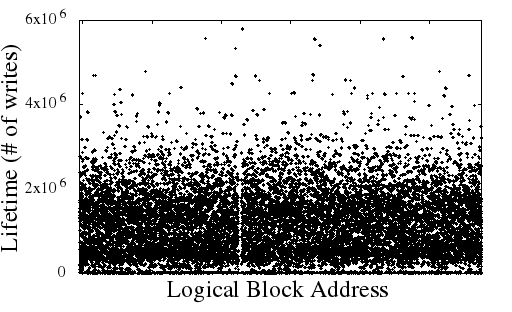
\includegraphics[width=0.215\textwidth]{figure/lba_lifetime2}}  % data from 0/03031641
	\hspace{10pt}
	\subfloat[Lifetime patterns over time]{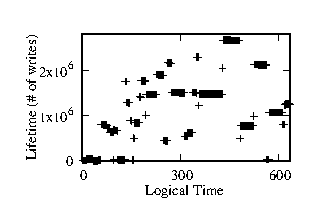
\includegraphics[width=0.21\textwidth]{figure/lifetime_in_chunk}}
	%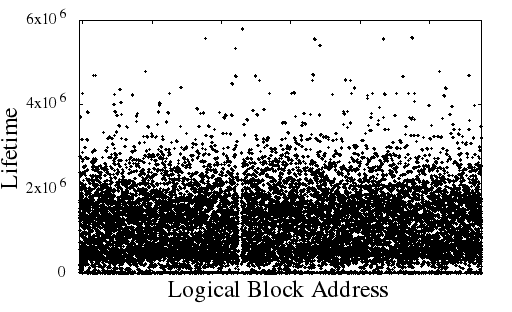
\includegraphics[width=0.9\linewidth]{figure/lba_lifetime} 
	%\vspace{-3pt}
	\caption{Lifetime distributions of append-only workload over addresses and times.} %shane part
	\label{fig:lba_lifetime}
	%\vspace{-20pt}
\end{figure}


We also analyzed 
if the lifetimes of LBAs change under some predictable patterns over time 
although the overall lifetime distribution shows large variances.
Fig.~\ref{fig:lba_lifetime}(b) shows a scatter plot of data lifetimes over the logical time 
for a specific 1-MB chunk with 256 pages. 
As shown in Fig.~\ref{fig:lba_lifetime}(b), 
for the given chuck, data lifetimes vary in a random fashion
(although some temporal locality is observed).
Over the logical time, the lifetime of data written to the chunk 
varies in an unpredictable fashion.  
For example, at the logical time 10, the lifetime was 1 but it increases about 
2.6 million around the logical time 450 
followed by a rapid drop around the logical time 600. 
Our illustration using RocksDB strongly suggests that under append-only
workloads, LBAs are not useful in deciding data lifetimes.
Therefore, we should find new information 
to predict data lifetimes in developing an automatic stream management techique.


\subsection{Limit to the Number of Streams}
It is advantageous to support a large number of streams in order to manage data with different lifetime characteristics as distinct streams.
As explained in ~\cite{MultiStream}, the performance continues to improve until 
the number of streams increases enough to distinguish the lifetime characteristics exists in the application.
Therefore, the multi-stream specification defines up to 65536 streams~\cite{T10, NVMe}.
However, the number of streams actually supported by an SSD that implements the specification is limited to 4 to 16~\cite{MultiStream, Level, AutoStream}.
This limitation occurs due to restrictions on the resource required to implement multi-stream. The requirement can be divided into memory, power, and overprovision resource.

First, memory resource may limit the number of multi-stream.
The controller that runs the SSD provides various memories such as TCM, SRAM, and DRAM. 
To optimize the performance, frequently referenced data structures should be located in fast memory.
The size of the data structure associated with a multi-stream is proportional to the number of streams supported and is directly related to performance, so it must be located in fast memory.
However, because of limited memory sizes, such as TCM or SRAM,
 there is a limit to the number of streams that can be supported with good performance.

Second, power resource may limit the number of multi-stream.
SSDs that support multi-stream are used in data centers or storage servers. SSDs use tantalum or electrolytic capacitors as backup power to guarantee data integrity even under sudden power off conditions.
Buffered data that is used to effectively utilize the parallelism of flash ensures reliable write to flash by using backup power during power off detection.
Since the buffered data is managed per stream, its size increases in proportion to the number of streams.
This also limits the number of streams that can be supported because SSDs use limited backup power at the limited PCB size.

Lastly, overprovision resource may limit the number of multi-stream.
As the number of multi-stream support increases, the active point increases. 
For each active point, it is necessary to allocate separate flash blocks.
 As the number of streams increases, it causes a decrease in overprovision area of SSD.
However, since the overprovisioning area of the SSD is limited, if the number of streams becomes too large, there may be a problem of increase of WAF due to overprovision reduction. 
In the case of streams over the number of overprovisioned blocks, flash block allocation  is not possible.
As a result, this makes stream mapping even more difficult.

